{\color{indiagreen}\subsection{Vodoravni met}}
\begin{center}
	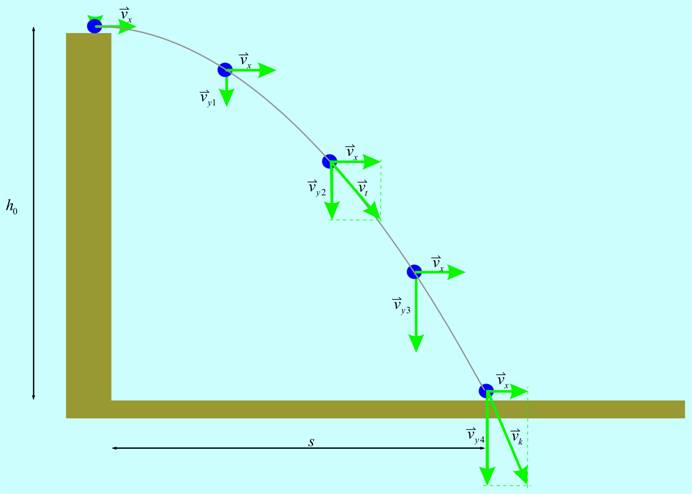
\includegraphics[width=15cm, height=15cm,keepaspectratio=true]{vodoravni_met.jpg}
\end{center}
Hitrost $\vec{v}$ je vedno \textbf{tangentna} na traektorijo(pot po kateri se premika).\\

\begin{center}
	\begin{tabular}{|c c|} 
 	\hline
 	X smer & Y smer \\
 	\hline
 	enakomerno gibanje & enakomerno pospešeno gibanje \\
 	v = konst. & a = g, v $\neq$ konst.\\
 	/ & prosti pad\\
 	t & t\\
 	\hline
 	\end{tabular}
\end{center}


\begin{align*}
	v_x &= \frac{x}{t}\\
	v &= \sqrt{v_x^2 + v_y^2}\\
	v_y &= gt\\
	h &= \frac{gt^2}{2}\\
\end{align*}